%package list
\documentclass{article}
\usepackage[top=3cm, bottom=3cm, outer=3cm, inner=3cm]{geometry}
\usepackage{multicol}
\usepackage{graphicx}
\usepackage{url}
%\usepackage{cite}
\usepackage{hyperref}
\usepackage{array}
%\usepackage{multicol}
\newcolumntype{x}[1]{>{\centering\arraybackslash\hspace{0pt}}p{#1}}
\usepackage{natbib}
\usepackage{pdfpages}
\usepackage{multirow}
\usepackage[normalem]{ulem}
\useunder{\uline}{\ul}{}
\usepackage{svg}
\usepackage{xcolor}
\usepackage{listings}
\lstdefinestyle{ascii-tree}{
    literate={├}{|}1 {─}{--}1 {└}{+}1 
  }
\lstset{basicstyle=\ttfamily,
  showstringspaces=false,
  commentstyle=\color{red},
  keywordstyle=\color{blue}
}
%\usepackage{booktabs}
\usepackage{caption}
\usepackage{subcaption}
\usepackage{float}
\usepackage{array}

\newcolumntype{M}[1]{>{\centering\arraybackslash}m{#1}}
\newcolumntype{N}{@{}m{0pt}@{}}


%%%%%%%%%%%%%%%%%%%%%%%%%%%%%%%%%%%%%%%%%%%%%%%%%%%%%%%%%%%%%%%%%%%%%%%%%%%%
%%%%%%%%%%%%%%%%%%%%%%%%%%%%%%%%%%%%%%%%%%%%%%%%%%%%%%%%%%%%%%%%%%%%%%%%%%%%
\newcommand{\itemEmail}{aquispearr@unsa.edu.pe}
\newcommand{\itemEmail}{pcaril@unsa.edu.pe}
\newcommand{\itemEmail}{jbasurcoc@unsa.edu.pe}

\newcommand{\itemStudentA}{Alexandra Raquel Quispe   } 
\newcommand{\itemStudentB}{Paul Andree Cari                    } 
\newcommand{\itemStudentC}{Jeferson Joao Basurco} 

\newcommand{\itemCourse}{Programación Web II}
\newcommand{\itemCourseCode}{20231001}
\newcommand{\itemSemester}{I}
\newcommand{\itemUniversity}{Universidad Nacional de San Agustín de Arequipa}
\newcommand{\itemFaculty}{Facultad de Ingeniería de Producción y Servicios}
\newcommand{\itemDepartment}{Departamento Académico de Ingeniería de Sistemas e Informática}
\newcommand{\itemSchool}{Escuela Profesional de Ingeniería de Sistemas}
\newcommand{\itemAcademic}{2024 - A}
\newcommand{\itemInput}{Del 18 Junio 2024}
\newcommand{\itemOutput}{Al 22 Junio 2023}
\newcommand{\itemPracticeNumber}{09}
\newcommand{\itemTheme}{Angular}
%%%%%%%%%%%%%%%%%%%%%%%%%%%%%%%%%%%%%%%%%%%%%%%%%%%%%%%%%%%%%%%%%%%%%%%%%%%%
%%%%%%%%%%%%%%%%%%%%%%%%%%%%%%%%%%%%%%%%%%%%%%%%%%%%%%%%%%%%%%%%%%%%%%%%%%%%

\usepackage[english,spanish]{babel}
\usepackage[utf8]{inputenc}
\AtBeginDocument{\selectlanguage{spanish}}
\renewcommand{\figurename}{Figura}
\renewcommand{\refname}{Referencias}
\renewcommand{\tablename}{Tabla} %esto no funciona cuando se usa babel
\AtBeginDocument{%
	\renewcommand\tablename{Tabla}
}

\usepackage{fancyhdr}
\pagestyle{fancy}
\fancyhf{}
\setlength{\headheight}{30pt}
\renewcommand{\headrulewidth}{1pt}
\renewcommand{\footrulewidth}{1pt}
\fancyhead[L]{\raisebox{-0.2\height}{
\includegraphics[width=3cm]{img/logo_episunsa.png}}}
\fancyhead[C]{\fontsize{7}{7}\selectfont	\itemUniversity \\ \itemFaculty \\ \itemDepartment \\ \itemSchool \\ \textbf{\itemCourse}}
\fancyhead[R]{\raisebox{-0.2\height}{
\includegraphics[width=1.2cm]{img/logo_abet}}}
\fancyfoot[L]{Quispe Alexandra - Cari Paul - Basurco Joao}
\fancyfoot[C]{\itemCourse}
\fancyfoot[R]{Página \thepage}

% para el codigo fuente
\usepackage{listings}
\usepackage{color, colortbl}
\definecolor{dkgreen}{rgb}{0,0.6,0}
\definecolor{gray}{rgb}{0.5,0.5,0.5}
\definecolor{mauve}{rgb}{0.58,0,0.82}
\definecolor{codebackground}{rgb}{0.95, 0.95, 0.92}
\definecolor{tablebackground}{rgb}{0.8, 0, 0}

\lstset{frame=tb,
	language=bash,
	aboveskip=3mm,
	belowskip=3mm,
	showstringspaces=false,
	columns=flexible,
	basicstyle={\small\ttfamily},
	numbers=none,
	numberstyle=\tiny\color{gray},
	keywordstyle=\color{blue},
	commentstyle=\color{dkgreen},
	stringstyle=\color{mauve},
	breaklines=true,
	breakatwhitespace=true,
	tabsize=3,
	backgroundcolor= \color{codebackground},
}

\begin{document}
	
	\vspace*{10px}
	
	\begin{center}	
		\fontsize{17}{17} \textbf{ Informe de Laboratorio \itemPracticeNumber}
	\end{center}
	\centerline{\textbf{\Large Tema: \itemTheme}}
	%\vspace*{0.5cm}	

	\begin{flushright}
		\begin{tabular}{|M{2.5cm}|N|}
			\hline 
			\rowcolor{tablebackground}
			\color{white} \textbf{Nota}  \\
			\hline 
			     \\[30pt]
			\hline 			
		\end{tabular}
	\end{flushright}	

	\begin{table}[H]
		\begin{tabular}{|x{4.7cm}|x{4.8cm}|x{4.8cm}|}
			\hline 
			\rowcolor{tablebackground}
			\color{white} \textbf{Estudiante} & \color{white}\textbf{Escuela}  & \color{white}\textbf{Asignatura}   \\
			\hline 
			{\itemStudentA 
   \itemStudentB
   \itemStudentC 
   \par } & \itemSchool & {\itemCourse \par Semestre: \itemSemester \par Código: \itemCourseCode}     \\
			\hline 			
		\end{tabular}
	\end{table}		
	
	\begin{table}[H]
		\begin{tabular}{|x{4.7cm}|x{4.8cm}|x{4.8cm}|}
			\hline 
			\rowcolor{tablebackground}
			\color{white}\textbf{Laboratorio} & \color{white}\textbf{Tema}  & \color{white}\textbf{Duración}   \\
			\hline 
			\itemPracticeNumber & \itemTheme & 12 horas   \\
			\hline 
		\end{tabular}
	\end{table}
	
	\begin{table}[H]
		\begin{tabular}{|x{4.7cm}|x{4.8cm}|x{4.8cm}|}
			\hline 
			\rowcolor{tablebackground}
			\color{white}\textbf{Semestre académico} & \color{white}\textbf{Fecha de inicio}  & \color{white}\textbf{Fecha de entrega}   \\
			\hline 
			\itemAcademic & \itemInput &  \itemOutput  \\
			\hline 
		\end{tabular}
	\end{table}
	
	\section{Tarea}
	\begin{itemize}		
Se desea crear un proyecto con Angular que implemente el juego del ahorcado.  Se tendrá un arreglo con posibles palabras a adivinar por parte del usuario.  La interfaz la dejamos a gusto de ustedes los programadores.
\begin{verbatim}
npm install -g @angular/cli    
\end{verbatim}
Alternativamente, se puede utilizar un servidor web como Apache con Xampp. Luego, se debe descargar el archivo \texttt{data.json} y colocarlo en el directorio raíz del servidor web.

Para cada problema propuesto, se debe implementar un programa en Ajax y una página que realice las siguientes tareas:

	\end{itemize}
		
\section{Equipos, materiales y temas utilizados}
\begin{itemize}
    \item \textbf{Sistema Operativo:} Ubuntu GNU/Linux 23.04 Lunar Lobster 64 bits, Kernel 6.2.
    \item \textbf{Editor de texto:} VIM 9.0.
    \item \textbf{Entorno de desarrollo:} OpenJDK 64-Bits 17.0.7.
    \item \textbf{Control de versiones:} Git 2.39.2.
    \item \textbf{Repositorio:} Cuenta en GitHub con el correo institucional.
    \item \textbf{Tecnologías utilizadas:}
    \begin{itemize}
        \item \textbf{Ajax:} Para la implementación de solicitudes asíncronas y la manipulación dinámica de datos.
        \item \textbf{Google Charts:} Para la visualización gráfica de datos, incluyendo gráficos de líneas y gráficos comparativos.
        \item \textbf{Python:} Utilizado para lanzar un servidor web local para pruebas.
        \item \textbf{Servidor web:} SimpleHTTPServer (Python 2) o http.server (Python 3) para el desarrollo y prueba de aplicaciones web.
    \end{itemize}
\end{itemize}

\section{URL de Repositorio GitHub}
\begin{itemize}
    \item URL del Repositorio GitHub para clonar o recuperar.
    \item \url{https://github.com/JefersonPWeb2/Pweb2-Lab09.git}
     \item Videos
    \item \url{ https://docs.google.com/document/d/13EKPi-5QbAI2lYFi6uTgnXr7N8dtd6rU0wayuecb0CE/edit}
   
    
\end{itemize}
\section{Actividades}
	
	\subsection{Actividad 1}
	\begin{itemize}	
		\item Creamos el directorio assets donde estaran las imagenes del ahorcado.
    \newline
         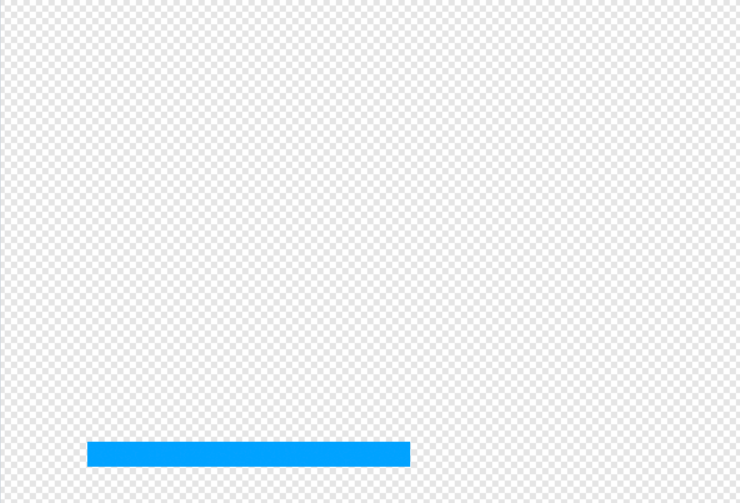
\includegraphics[width=0.25\linewidth]{imagen - 1.png}  
           \newline
         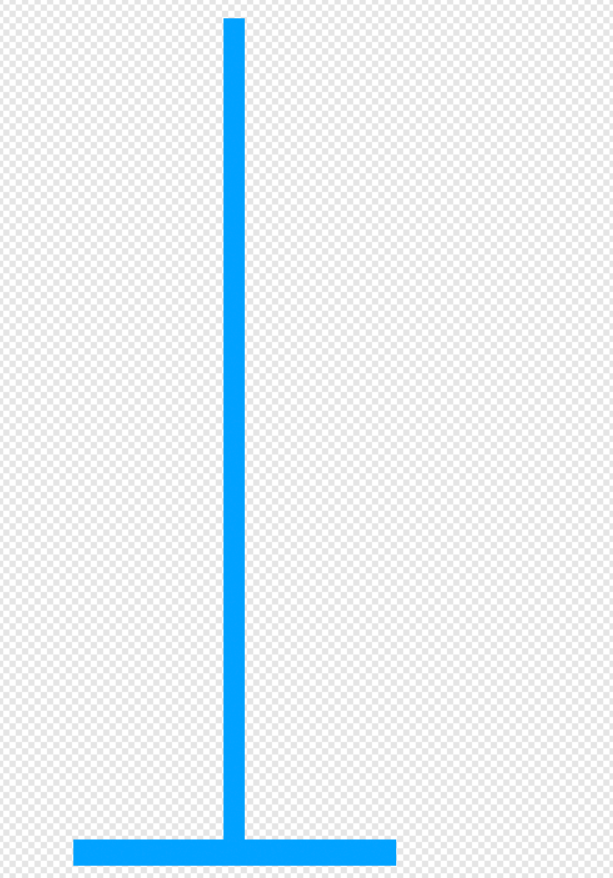
\includegraphics[width=0.25\linewidth]{imagen - 2.png}  
           \newline
         
\includegraphics[width=0.25\linewidth]{imagen - 3.png} 
           \newline
         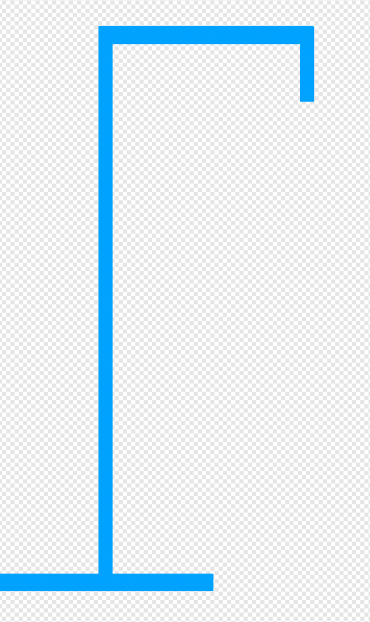
\includegraphics[width=0.25\linewidth]{imagen - 4.png} 
           \newline
         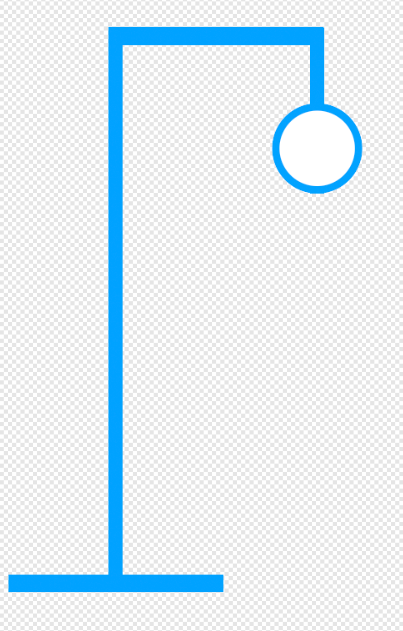
\includegraphics[width=0.25\linewidth]{imagen - 5.png} 
           \newline
         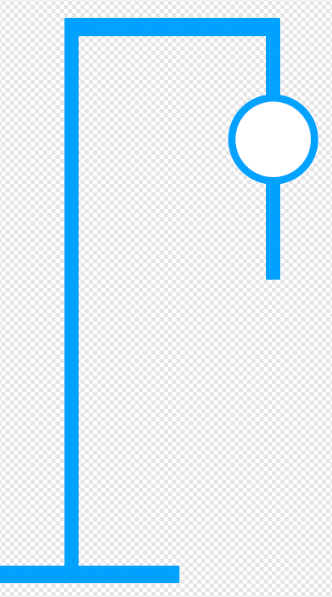
\includegraphics[width=0.25\linewidth]{imagen - 6.png} 
           \newline
         
\includegraphics[width=0.25\linewidth]{imagen - 7.png}  
           \newline
         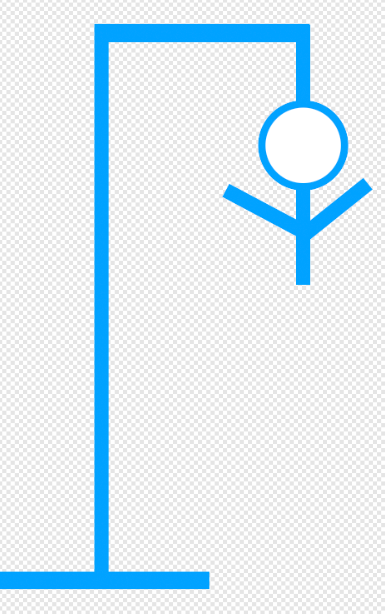
\includegraphics[width=0.25\linewidth]{imagen - 8.png} 
           \newline
         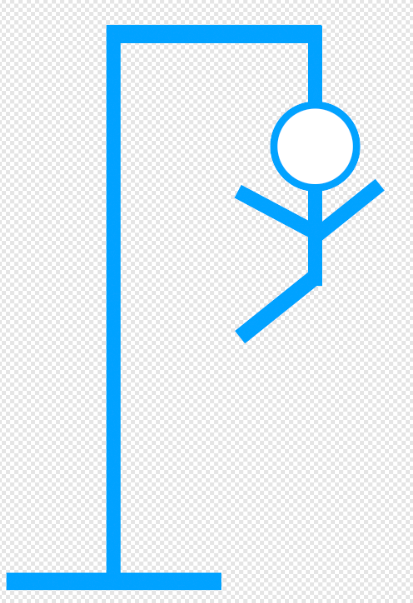
\includegraphics[width=0.25\linewidth]{imagen - 9.png} 
           \newline
         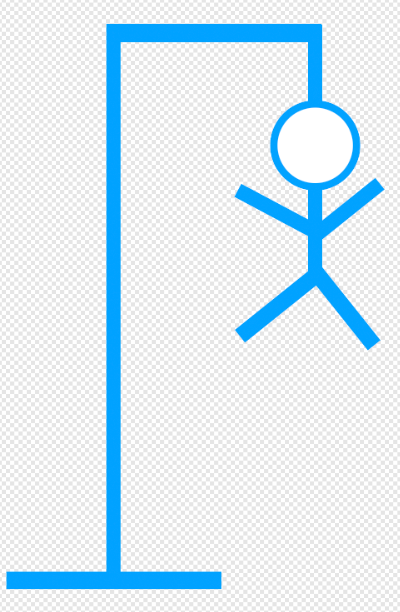
\includegraphics[width=0.25\linewidth]{imagen -10.png}  
      
    \newline
        \newline
	\end{itemize}	
           
       \subsection{Actividad 2}
	\begin{itemize}	
		\item Creación de un alfabeto, método adivinar, mensaje final y reinicio del juego
	\end{itemize}
         
 
    \lstinputlisting[language=TypeScript]{Actividad1.ts}
        
     \subsection{Actividad 3}
       \begin{itemize}	
		\item Configurando la carpeta assets para incluir la carpeta hangman
             \end{itemize}
             \centering
        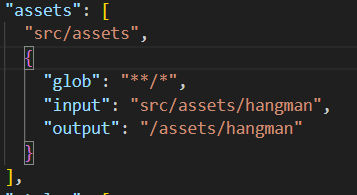
\includegraphics[width=0.40\linewidth]{Actividad 2.png}  
        
          \subsection{Actividad 4}
	\begin{itemize}	
		\item Modificando el html de game-board para que muestre botones del alfabeto y mensajes de juego
	\end{itemize}
        \lstinputlisting[language=HTML]{game-board.component.html}

        
         \subsection{Actividad 5}
	\begin{itemize}	
		\item Agregando css al componente
	\end{itemize}
 \centering
        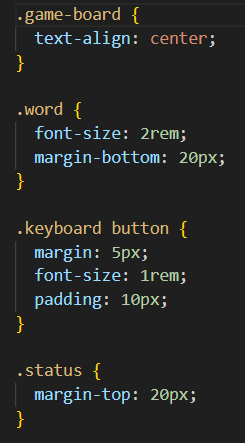
\includegraphics[width=0.40\linewidth]{Actividad 5.png}  
        
        
        \subsection{Actividad 6}
	\begin{itemize}	
		\item Creación de constructor y metodo getImagenURL para retornar una ruta 
  
	\end{itemize}
        \lstinputlisting[language=TypeScript]{hangman-figure.component.ts}

    \subsection{Actividad 7}
	\begin{itemize}	
		\item Mostrando imagen del ahorcado en la interfaz
	\end{itemize}
           \lstinputlisting[language=HTML]{ hangman-figure.component.html}
       
    \subsection{Actividad 8}
         \begin{itemize}	
		\item Agregando css al componente
	\end{itemize}
 \centering
   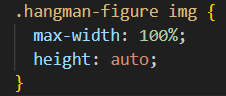
\includegraphics[width=0.45\linewidth]{Actividad 8.png} 
   
      \subsection{Actividad 9}
         \begin{itemize}	
		\item Cambiando número de intentos
	\end{itemize}
   \lstinputlisting[language=TypeScript]{palabras.service.ts}  
          
     \subsection{Actividad 10}
         \begin{itemize}	
		\item Importando los componentes e inicializando el número de intentos
	\end{itemize}
  \lstinputlisting[language=TypeScript]{app.component.ts}  
 




\begin{figure}[htbp]
\section{Resultados}
    \centering
    \begin{minipage}{1\textwidth}
        \centering
        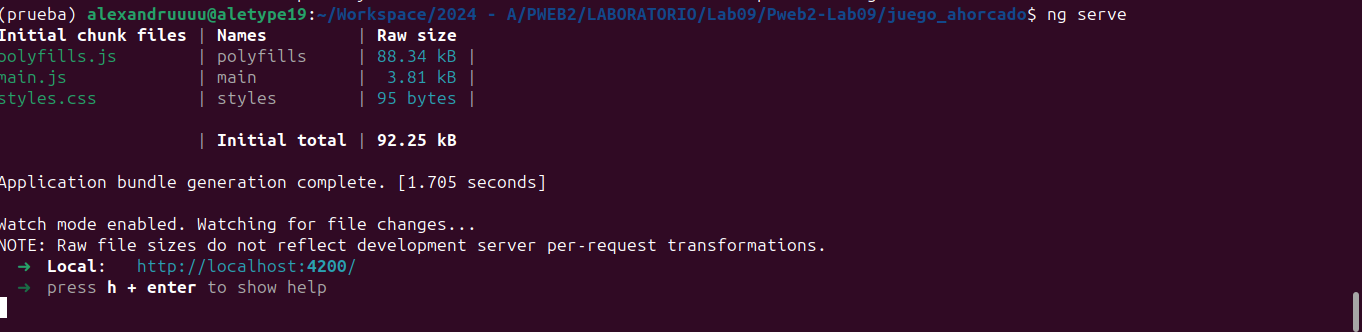
\includegraphics[width=0.9\textwidth]{img/resul1.png}
        \caption{Iniciando el servidor de desarrollo de Angular}
        \label{fig:resul1}
    \end{minipage}
    \vspace{1cm}
    \begin{minipage}{1\textwidth}
        \centering
        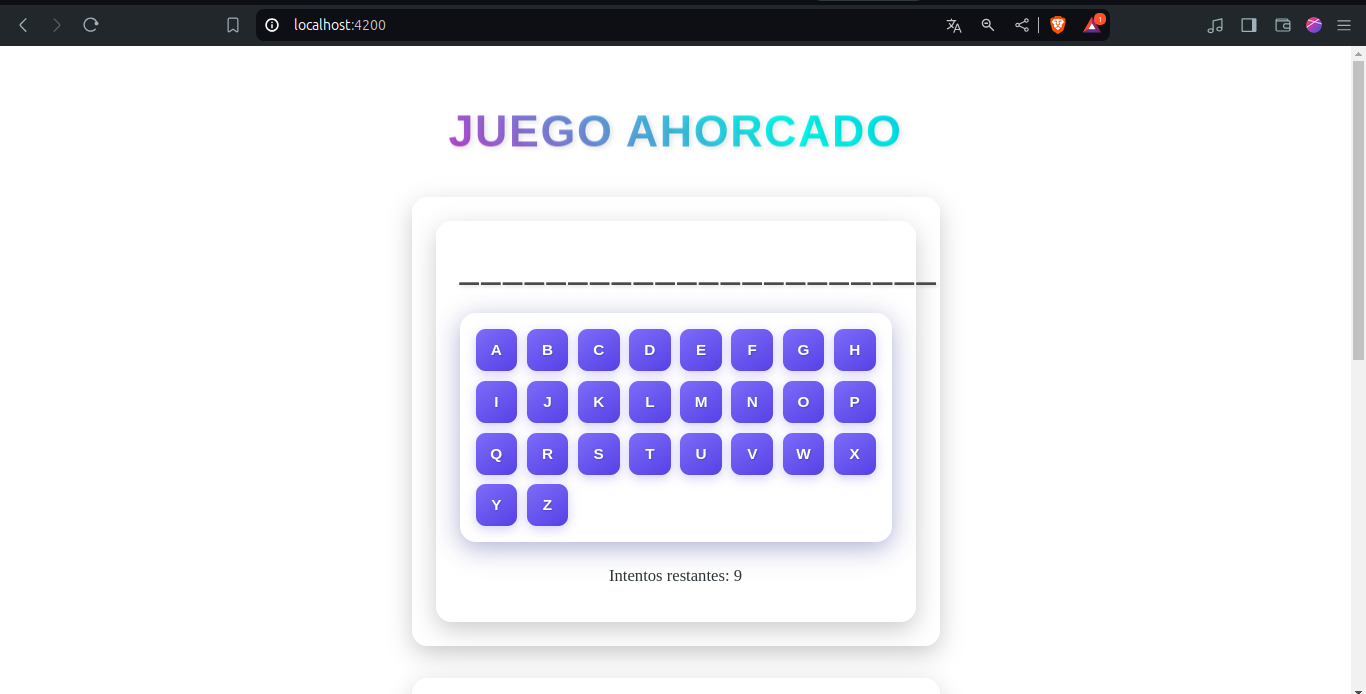
\includegraphics[width=0.9\textwidth]{img/reult2.png}
        \caption{Resultado final del juego}
        \label{fig:enter-label2}
    \end{minipage}
    \vspace{1cm}
    \begin{minipage}{1\textwidth}
        \centering
        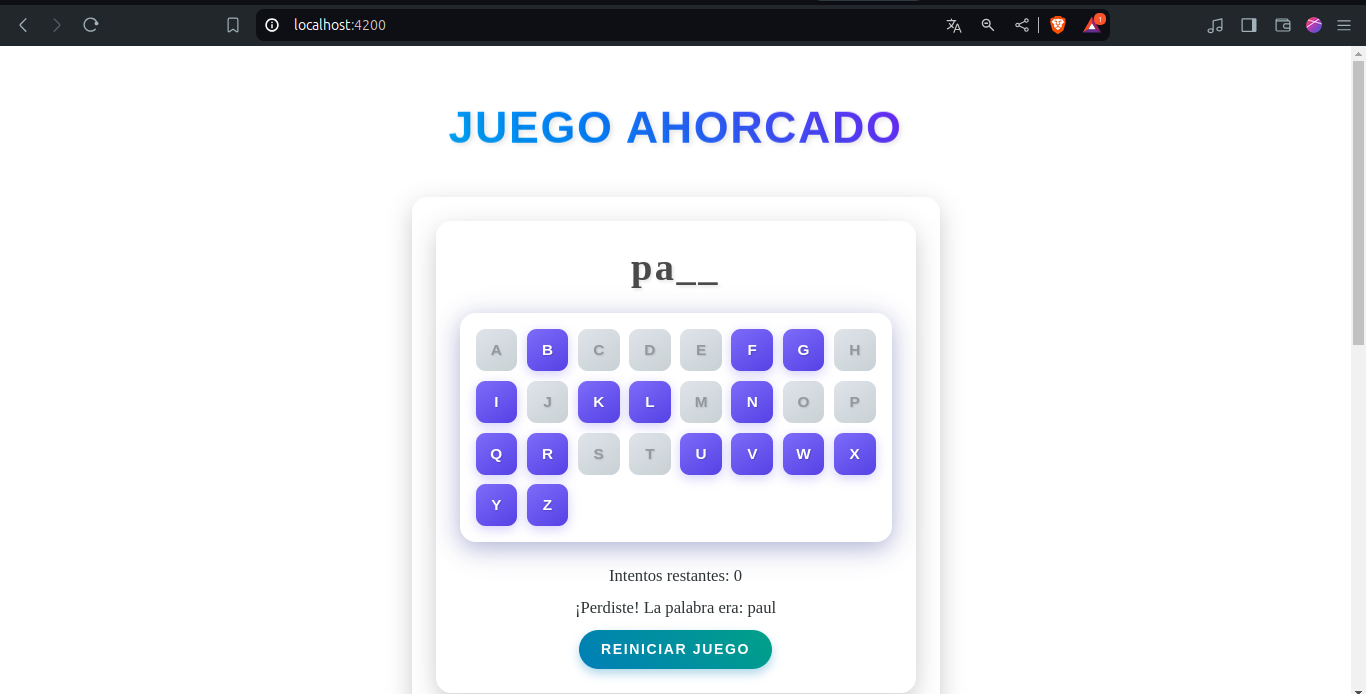
\includegraphics[width=0.9\textwidth]{img/result2.png}
        \caption{Resultado final del juego}
        \label{fig:result2}
    \end{minipage}
    \vspace{1.5cm}

\end{figure}
    \begin{minipage}{1\textwidth}
        \centering
        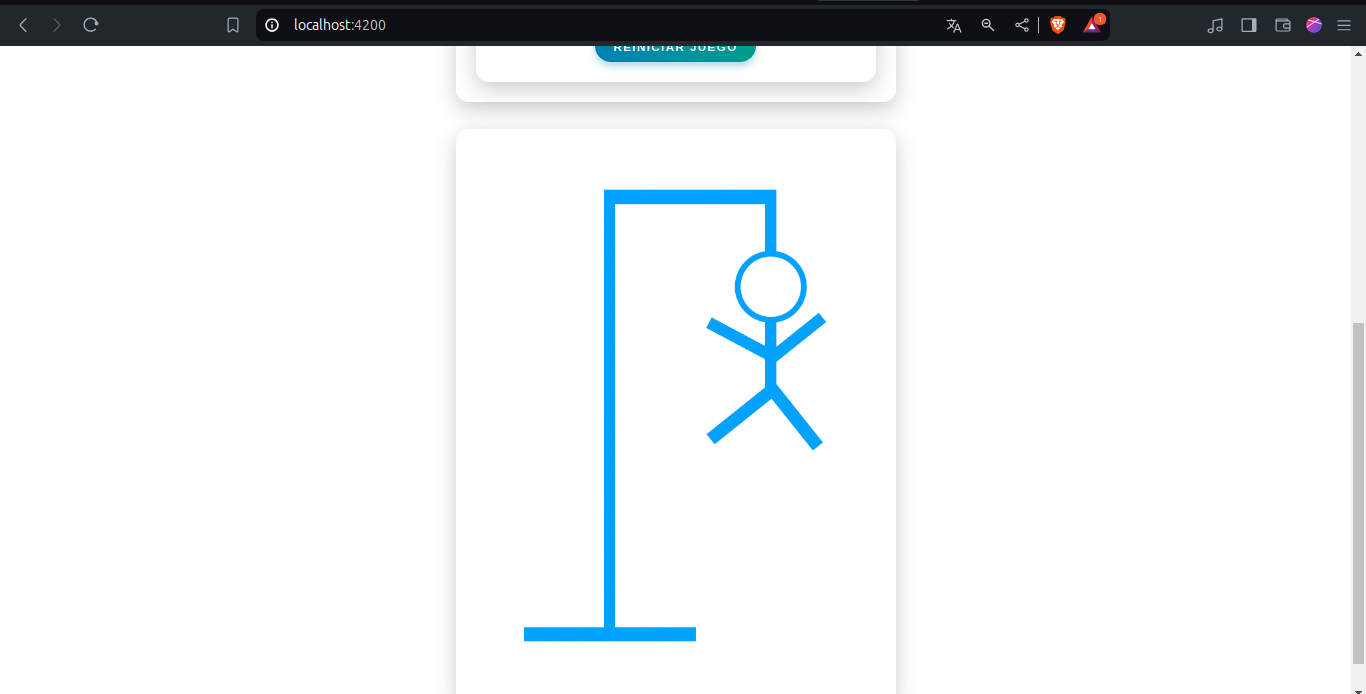
\includegraphics[width=1\textwidth]{img/result3.png}
        \caption{Resultado final del juego}
        \label{fig:result3}
    \end{minipage}



\clearpage
%%%%%%%%%%%%%%%%%%%%%%%%%%%%%%%%%%%%%%%%%%%%%%%%%%%%%%%%%%%%%%%%%%%%%%%%%%%%%%%%%%%%%%%%%%%%%%%%%%%%%%%%%
%%%%%%%%%%%%%%%%%%%%%%%%%%%%%%%%%%%		


	
\subsection{\textcolor{red}{Rúbrica para el contenido del Informe y demostración}}
	\begin{itemize}			
		\item El alumno debe marcar o dejar en blanco en celdas de la columna \textbf{Checklist} si cumplio con el ítem correspondiente.
		\item Si un alumno supera la fecha de entrega,  su calificación será sobre la nota mínima aprobada, siempre y cuando cumpla con todos lo items.
		\item El alumno debe autocalificarse en la columna \textbf{Estudiante} de acuerdo a la siguiente tabla:
	
		\begin{table}[ht]
			\caption{Niveles de desempeño}
			\begin{center}
			\begin{tabular}{ccccc}
    			\hline
    			 & \multicolumn{4}{c}{Nivel}\\
    			\cline{1-5}
    			\textbf{Puntos} & Insatisfactorio 25\%& En Proceso 50\% & Satisfactorio 75\% & Sobresaliente 100\%\\
    			\textbf{2.0}&0.5&1.0&1.5&2.0\\
    			\textbf{4.0}&1.0&2.0&3.0&4.0\\
    		\hline
			\end{tabular}
		\end{center}
	\end{table}	
	
	\end{itemize}
	
	\begin{table}[H]
		\caption{Rúbrica para contenido del Informe y demostración}
		\setlength{\tabcolsep}{0.5em} % for the horizontal padding
		{\renewcommand{\arraystretch}{1.5}% for the vertical padding
		%\begin{center}
		\begin{tabular}{|p{2.7cm}|p{7cm}|x{1.3cm}|p{1.2cm}|p{1.5cm}|p{1.1cm}|}
			\hline
    		\multicolumn{2}{|c|}{Contenido y demostración} & Puntos & Checklist & Estudiante & Profesor\\
			\hline
			\textbf{1. GitHub} & Hay enlace URL activo del directorio para el  laboratorio hacia su repositorio GitHub con código fuente terminado y fácil de revisar. &2 &X &2 & \\ 
			\hline
			\textbf{2. Commits} &  Hay capturas de pantalla de los commits más importantes con sus explicaciones detalladas. (El profesor puede preguntar para refrendar calificación). &4 &X &2 &  \\ 
			\hline 
			\textbf{3. Código fuente} &  Hay porciones de código fuente importantes con numeración y explicaciones detalladas de sus funciones. &2 &X &1 & \\ 
			\hline 
			\textbf{4. Ejecución} & Se incluyen ejecuciones/pruebas del código fuente  explicadas gradualmente. &2 &X &1 & \\ 
			\hline			
			\textbf{5. Pregunta} & Se responde con completitud a la pregunta formulada en la tarea.  (El profesor puede preguntar para refrendar calificación).  &2 &X &2 & \\ 
			\hline	
			\textbf{6. Fechas} & Las fechas de modificación del código fuente estan dentro de los plazos de fecha de entrega establecidos. &2 &X &2 & \\ 
			\hline 
			\textbf{7. Ortografía} & El documento no muestra errores ortográficos. &2 &X &2 & \\ 
			\hline 
			\textbf{8. Madurez} & El Informe muestra de manera general una evolución de la madurez del código fuente,  explicaciones puntuales pero precisas y un acabado impecable.   (El profesor puede preguntar para refrendar calificación).  &4 &X &3 & \\ 
			\hline
			\multicolumn{2}{|c|}{\textbf{Total}} &20 & &15 & \\ 
			\hline
		\end{tabular}
		%\end{center}
		%\label{tab:multicol}
		}
	\end{table}
	
\clearpage



	
%\clearpage
%\bibliographystyle{apalike}
%\bibliographystyle{IEEEtranN}
%\bibliography{bibliography}
			
\end{document}
